\section{Experimental Setup}
\label{sec:setup}

\paragraph{Data.}
We use two sorting tasks. \emph{SMS smishing} uses the UCI SMS Spam Collection
(5{,}574 messages, 747 labelled spam), with spam treated as malicious. The task
label is therefore ``SMS spam/smishing''; the collection's spam class is mostly
scam and prize messages rather than messages that steal passwords, and we state
that as a limit on what the label means instead of hiding it.
\emph{Phishing email} uses the \texttt{zefang-liu/phishing-email-dataset} text
column, filtered to messages between 16 and 3{,}000 characters and
balanced-sampled to 1{,}000 benign and 1{,}000 phishing rows with a fixed seed.

\paragraph{Splits.}
The evaluation split is balanced and frozen: 200 benign and 200 malicious rows
per task, 800 rows in total, drawn with seed 42. The split is identical in every
run, and its hash is checked by the artefact's setup step, so a run that uses
different data fails before it can report a number. Attacks are launched on the
caught subset \emph{of this evaluation split}, which is a within-sample design:
the same 800 rows supply both the baseline and the attack set. We say so because
it means the ASR is not an out-of-sample estimate; it is a conditional
measurement on the messages the model got right, which is what Rule~1 defines.

\paragraph{Models.}
We evaluate three open instruction-tuned models, none compressed at inference:
Qwen2.5-3B-Instruct, SmolLM2-1.7B-Instruct and Phi-3.5-mini-instruct (3.8B). A
fourth model, Llama-3.2-3B-Instruct, was planned but sits behind a licence
acceptance and is not part of any number reported here.

\paragraph{Inference.}
All models are served behind one OpenAI-compatible endpoint and queried with the
same list of messages. Generation is greedy (temperature 0), capped at 8 new
tokens, with a single-word answer parser that returns malicious, benign, or
\emph{unparsed}; unparsed answers are counted separately and never guessed. In
the runs reported here, no answer failed to parse. Models are loaded at half
precision on one T4 GPU with automatic device placement.

\paragraph{Compute and cost.}
One full run --- clean baseline on 800 rows for three models, construction of the
attack set, and both attack modes for all three models --- takes 37.1 minutes on
a single free-tier T4. The reporting step is a separate pass over the per-sample
CSVs and runs on CPU.

\paragraph{Evaluation pipeline.}
Figure~\ref{fig:pipeline} shows the full pipeline. A message is classified by the
model. If the verdict is malicious, the message enters the attack set. The
perturbation engine applies edits and re-queries the model. The results are then
evaluated for transfer to other models and for defences.

\begin{figure}[t]
\centering
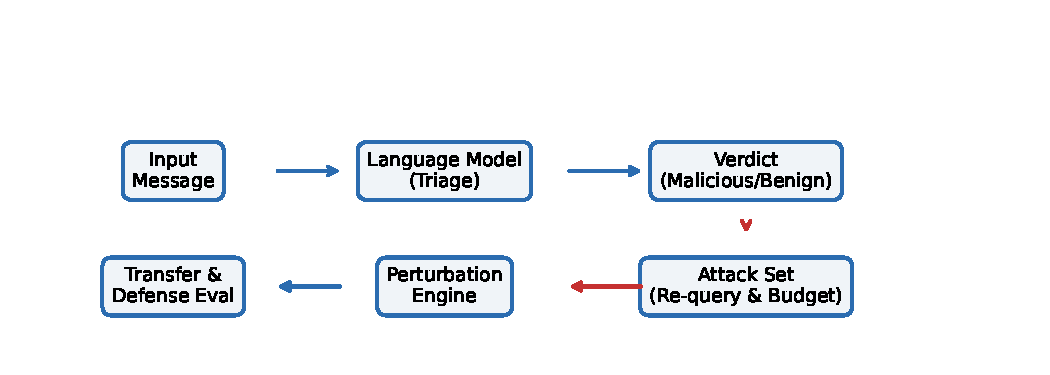
\includegraphics[width=\columnwidth]{figures/fig_pipeline}
\caption{The evaluation pipeline. A clean message is classified by the model. If the verdict is malicious, the message enters the attack set. The perturbation engine applies edits under budget and re-queries the model. The results are then evaluated for transfer and defense robustness.}
\label{fig:pipeline}
\end{figure}


\paragraph{Reproducibility.}
Splits, prompt, decoding and per-sample perturbation seeds are fixed. The study
was run twice from start to finish (two independent GPU sessions); comparing the
two runs sample by sample, joined on sample id, gives identical attacked ids and
identical success flags in all six result files, with differences only in empty
cells of the excluded rows. The second run is the one whose outputs are reported
here.
